\documentclass{article}

\usepackage{graphicx}
\usepackage{amsmath}
\usepackage{times}
	
\title{Design \& Professional Skills --- First Assignment}	
\author{}
\date{}
	
\begin{document}

\maketitle

\section*{Instructions}

The following exercises are intended just to get you started with
Python.  At the very least, you must complete the prerequisites during
week 1.  If you've programmed in python before, you can probably skip
the first few exercises.  If you've not programmed in python before,
get as far as you can, but we don't expect you to complete everything.

\textbf{This assignment is not assessed, but you do need to hand it in
  via Moodle by Monday 12th October at 12 noon so we can see how you've
  got on.  Feel free to collaborate with other students, but list who
  you have collaborated with in your submission.}

\section*{Prerequisite 1}

Install python 3.8 on the machine you intend to use to do your
coursework.  If you have problems, come to one of the ENGF0002
programming clinics at 1pm each day (see Moodle for link).

\section*{Prerequisite 2}

Install git on your machine.  This will allow you to check out
software and slides from github.  Familiarise yourself with the basics
of checking out and updating from a repository.

\section*{Prerequisite 3}

Ensure you can run tkinter packages using your python 3 installation,
as we'll need these for next week's assignments.  Tkinter usually
comes pre-installed with python installations, but in some cases you'll need to
install a separate package.

\vspace{0.1in}\noindent Test your install by checking out\\
\texttt{mhandley/ENGF2-2019/assignments/assignment1/tkinter\_test.py}\\
from github and checking it runs properly.

\vspace{0.1in}\noindent From the command line, if python is installed as python3, you can run this as:\\
\texttt{python3 tkinter\_test.py}

\section*{Exercise 1: GCD example from class}

\textbf{Type in} the GCD example from gcd-function.png in the git
respository and get it to run.  We'll cover this algorithm in more
detail in video 3 and explain how it works.

\vspace{0.1in} Why type it in, rather than cut and paste, or checkout
from github?  Simply, we want you to get set up with an appropriate
editor, and understand the very basics of python. If you type it in,
you'll remember it.  Likely you'll mistype something, and have to
understand what python's error messages are telling you.  And at the
least, you'll need to get to grips with python's use of whitespace to
indicate semantic grouping of statements.  Doing this with code where
you know what the answer should be is useful if you've not programmed
in python before.

\section*{Exercise 2: Odd or Even}

Write a program that asks the user for a number. Depending on whether
the number is even or odd, print out an appropriate message to the
user.

\vspace{0.1in}\noindent Hint: The python3 \texttt{input()} function will read input from the keyboard,
but in python3 the result will be a text string, not an integer.  You
may need to use the \texttt{int()} function to convert it to an integer type.

\section*{Exercise 3: Fizzbuzz}

Write a program that prints the numbers from 1 to 100. But for
multiples of three print ``Fizz'' instead of the number and for the
multiples of five print ``Buzz''. For numbers which are multiples of
both three and five print ``FizzBuzz''.

This is one of those classic interview questions that are supposed to
distinguish candidates that can program from those than cannot.  There
are lots of versions of FizzBuzz online, but we'd like you to attempt
your own before you go hunting for online solutions.

\vspace{0.1in}\noindent Hint: modular arithmetic might be useful.

\vspace{0.1in}\noindent Hint: you can do this with a \texttt{while} loop, as in the GCD example, but it's
more elegant to use a \texttt{for} loop and \texttt{range} operator.

\newpage
\section*{Exercise 4: Calculating Pi}

We want to compute an approximation of $\pi$ (3.141592...) up to a
 certain precision. One way to do this is by using a \emph{Monte Carlo
 method} as follows. Consider the square of edge length 1 and the
 circle of radius 1/2 inscribed in the square, as depicted
 below. Generate random points within the square. Suppose
 $N_{\text{hits}}$ points hit the circle, out of a total of
 $N_{\text{tot}}$ points.


\begin{center}
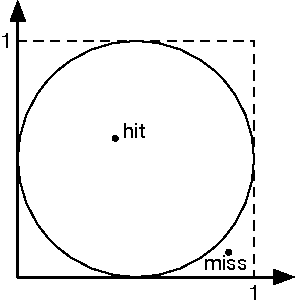
\includegraphics{ex1}
\end{center}

Then we can approximate $\pi$ by noting that $N_{\text{hits}}$
 estimates the area of the circle and $N_{\text{tot}}$ estimates the
 area of the square. In fact, recalling that the area of the circle is
 $\pi r^2$, for $r=1/2$ we have
\[
	\frac{A_{\text{circle}}}{A_{\text{square}}} = \frac{\pi}{4} \approx \frac{N_{\text{hits}}}{N_{\text{tot}}}
\]
%
Implement a function \texttt{estimate\_pi(precision)} that returns an
 approximation of $\pi$ up to \texttt{precision} decimal
 positions. Use the function \texttt{random()} from the module
 \texttt{random} to generate random numbers between $0$ and
 $1$. (\textbf{Hint:} the more points you generate, the more precise
 your approximation will be.)


\section*{Exercise 5: Breaking Caesar's Cipher}

A \emph{simple substitution cipher} is an encryption method where each letter of the alphabet is replaced by another one, according to a ciphertext alphabet. The Caesar's Cipher is a very simply substitution cipher, where each letter is replaced by one $n$ places later in the alphabet, wrapping back from Z to A if necessary.
For instance, in the cipher
\begin{verbatim}
    A B C D E F G H I J K L M N O P Q R S T U V W X Y Z    (original alphabet)
    N O P Q R S T U V W X Y Z A B C D E F G H I J K L M    (ciphertext alphabet)
\end{verbatim}
\texttt{A} is replaced by \texttt{N}, \texttt{B} by \texttt{O} and so on. Applying this cipher to the word \texttt{HELLO} produces the word \texttt{URYYB}. 

Implement a function \texttt{break\_cipher(text)} that takes a string
-- which is assumed to be encrypted using a Caesar cipher -- finds the
ciphertext alphabet used to encrypt it and returns the decrypted
string. Assume that the decrypted string will be in English, with
letters A-Z and no spaces.

As there are only 26 possible Caesar's Ciphers, you can easily break
them by hand.  But how would a program automatically decide which of the 26 possible
offsets is the correct one?

\end{document}
